\section{Question 3}

\subsection{The Question}

\begin{flushleft}

 Cluster the blogs using K-Means, using k=5,10,20. (see slide 18).
How many interations were required for each value of k?

\end{flushleft}
\subsection{The Answer}

The Python function used to produce the K-Means is provided in the book \cite{PCI}. Clustering into 5 clusters required 7 iterations. Clustering into 10 clusters required 6 iterations. Clustering into 20 clusters required 6 iterations.  The terminal output for the script is provided and displays that cluster members


\lstset{
    language=Python,
    label=code:q1,
    caption={Python script to produce dendrograms}
}
\lstinputlisting{../q3/q3.py}


\begin{figure}
\centering
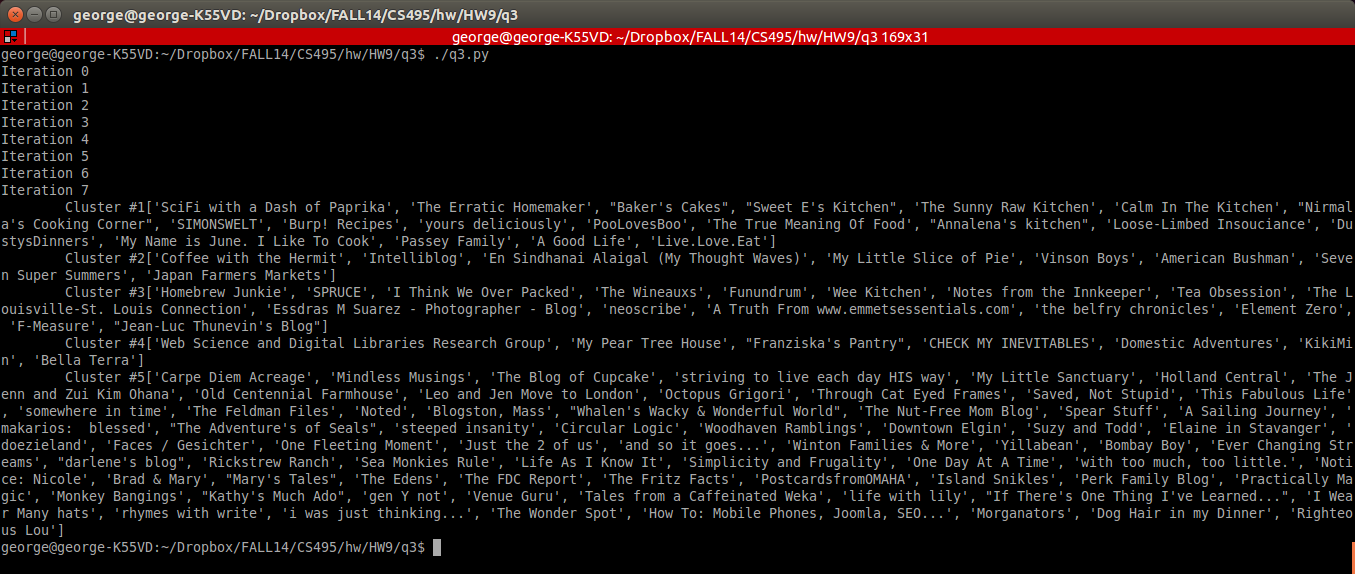
\includegraphics[width=\textwidth]{../q3/clust5.png}
\caption{Terminal output from K-Means CLustering, k = 5}
\end{figure}


\begin{figure}
\centering
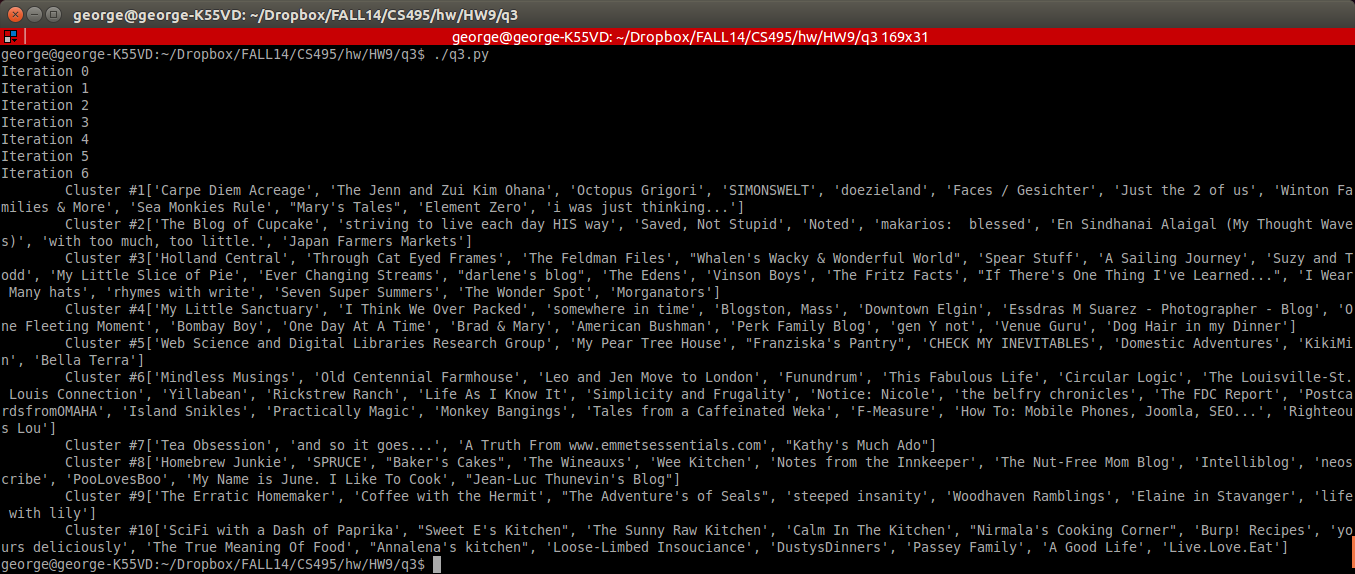
\includegraphics[width=\textwidth]{../q3/clust10.png}
\caption{Terminal output from K-Means CLustering, k = 10}
\end{figure}

\begin{figure}
\centering
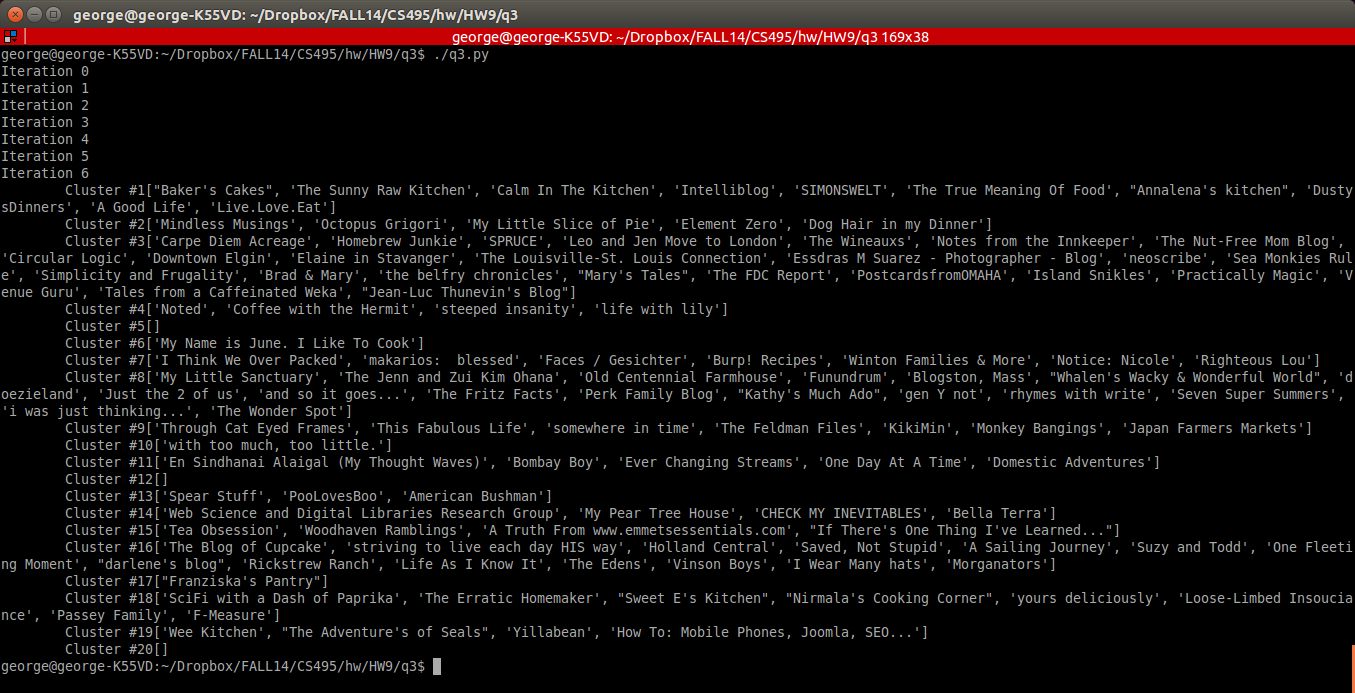
\includegraphics[width=\textwidth]{../q3/clust20.png}
\caption{Terminal output from K-Means CLustering, k = 20}
\end{figure}



